\clearpage
\section{Methods}
\label{sec.methods}

Schema of the proposed method is illustrated in Fig.~\ref{fig.schema}. There are five major stages in this method, including 

\begin{figure}[!h]
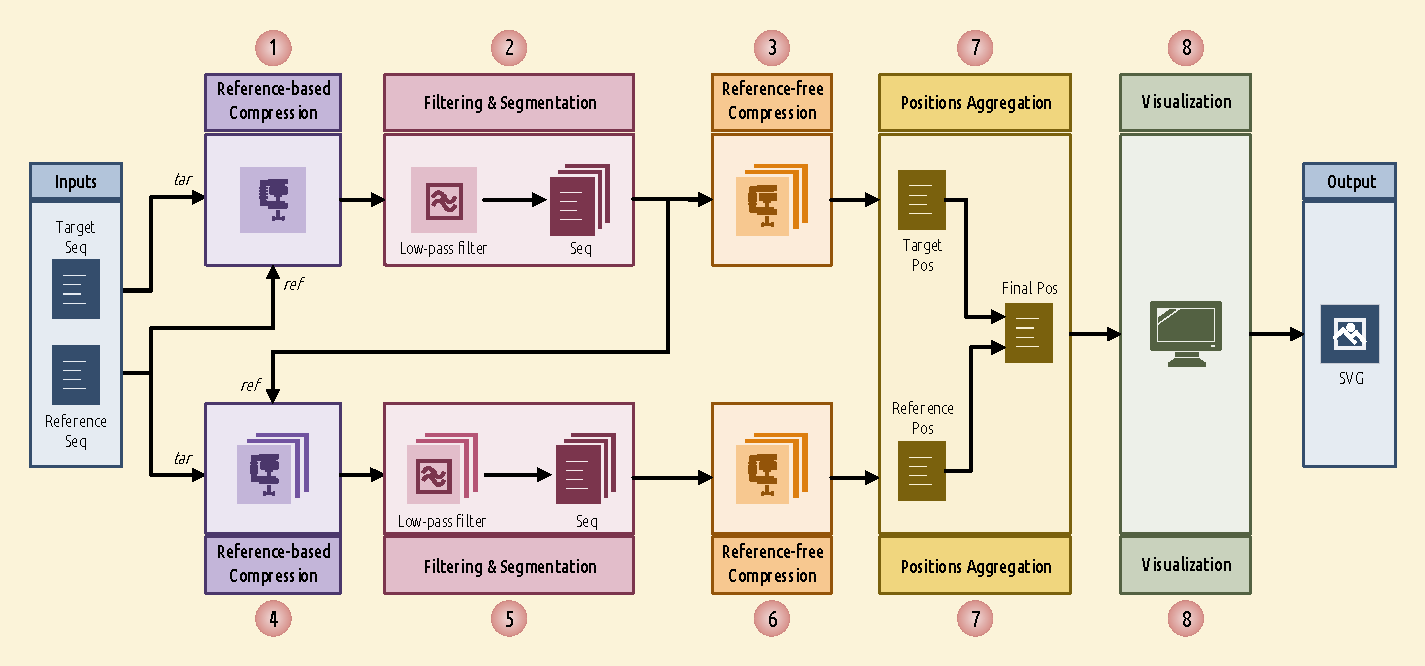
\includegraphics[width=\linewidth]{schema.pdf}
\caption{The schema of Smash++.}
\label{fig.schema}
\end{figure}

\subsection{Building models of the data}

\subsection{finding similar regions}

In order to smooth the profile information, we use Hann window, which is a discrete window function given by
\begin{equation}
  \label{eq.hann}
  w[n]=0.5-0.5\;\cos \left({\frac {2\pi n}{N}}\right)=\sin ^{2}\left({\frac {\pi n}{N}}\right),
\end{equation}
in which, $0\le n\le N$ and length of the window is $N+1$ (Fig.~\ref{fig.hann}).
\begin{figure}[!h]
  \centering
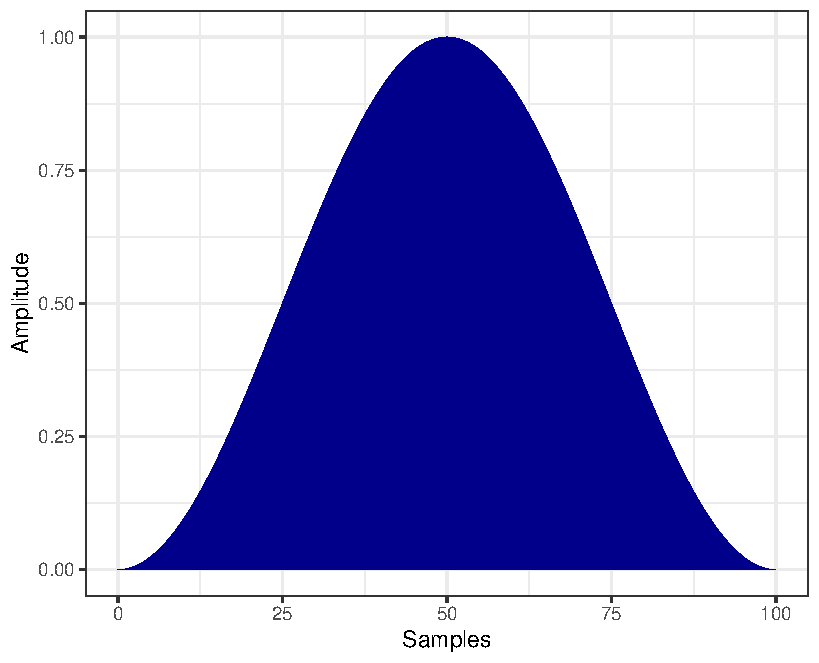
\includegraphics[width=7cm]{hann.pdf}
\caption{Hann window for 101 samples.}
\label{fig.hann}
\end{figure}

\subsection{Computing complexities}

\subsection{The software}

Besides Hann window, that is used as default to filter the profile information obtained by the reference-based compression, we have implemented several other window functions (Fig.~\ref{fig.filters}), including Blackman, Hamming, Nuttall, rectangular, sine, triangular and Welch windows. These functions are given by
\begin{align}
  w[n] &= 1,
  \tag*{(rectangular)} \\
  w[n] &= 1-\left|\tfrac {n-N/2}{L/2}\right|, \quad L=N,
  \tag*{(triangular/Bartlett)} \\
  w[n] &= 1-\left(\tfrac {n-N/2}{N/2}\right)^{2},
  \tag*{(Welch)} \\
  w[n] &= \sin \left(\tfrac {\pi n}{N}\right),
  \tag*{(sine)} \\
  w[n] &= 0.54348-0.45652\;\cos \left(\tfrac {2\pi n}{N}\right),
  \tag*{(Hamming)} \\
  w[n] &= 0.42659-0.49656\;\cos \left(\tfrac {2\pi n}{N}\right)+0.07685\;\cos \left(\tfrac {4\pi n}{N}\right),
  \tag*{(Blackman)} \\
  w[n] &= 0.35577-0.48740\;\cos \left(\tfrac {2\pi n}{N}\right)+0.14423\;\cos \left(\tfrac {4\pi n}{N}\right)-0.01260\;\cos \left(\tfrac {6\pi n}{N}\right).
  \tag*{(Nuttall)} \\
\end{align}

\begin{figure}[!h]
  \centering
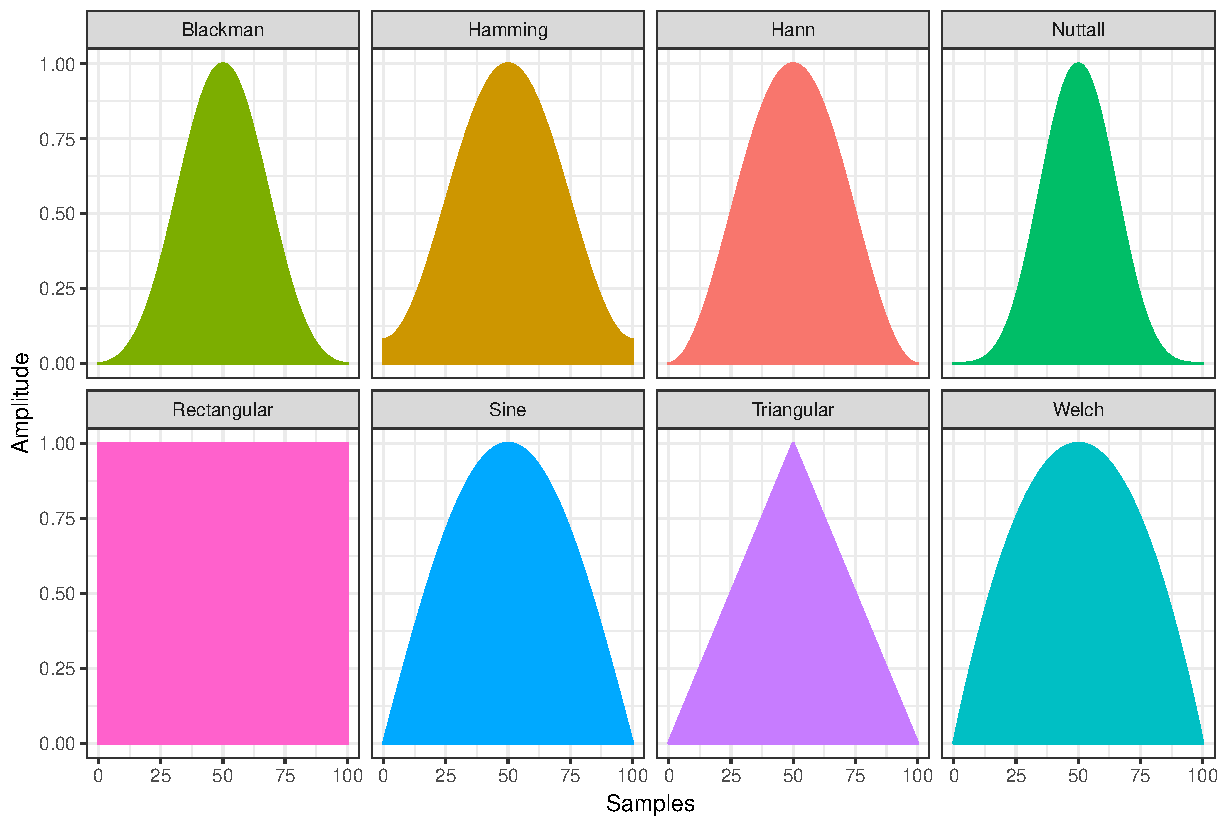
\includegraphics[width=.95\linewidth]{filters.pdf}
\caption{Window functions.}
\label{fig.filters}
\end{figure}
